\documentclass{article} % For LaTeX2e
\usepackage{url}
\usepackage[
style=authoryear,
backend=biber,
]{biblatex}
\usepackage{graphicx}
\graphicspath{ {./Graphics/} }
\usepackage{enumitem}

\addbibresource{ProposalBib.bib}

\title{Proposal Draft}
\author{
Adam Dameron 2
}

\begin{document}


\maketitle

\begin{abstract}
This proposal is for a project which seeks to use machine learning and object oriented statistics to model international human trafficking behavior. The goal of this project is to show which aspects of trafficking are most correlated with changes in a nations development. This is for the purposes of informing law enforcement and policy makers of what characteristics to be searching for.
\end{abstract}

\section{Introduction}
	Human trafficking occurs on a global scale, and has been recorded as an international concern since the year 1913 \parencite{Aromaa2007}. Many attempts have been made at defining it, yet these definitions remain unclear and vary greatly. The United Nations defines human trafficking as “recruitment, transportation, transfer, harboring or receipt of people through force, fraud or deception, with the aim of exploiting them for profit” \parencite{Raymond2002}. Human trafficking is strongly believed to occur in every country, and victimizes individuals of all ages, genders, and backgrounds \parencite{JacK2012}.\medskip
	
	A major gap in the global understanding of international human trafficking, is in how human trafficking is effected by changes in a country's economic and social development. The United Nations mentions this fact in its "Introduction to Human Trafficking," and describes trafficking as a "multidimensional problem," where a development is applicable \parencite{kangaspunta_2008}. However, there exists very little quantitative analysis into how trafficking and development are connected. This research seeks to provide more insight into what connections exist, if any.
	
	%Possibly Redundant%
	%Despite mounting global concern, there still exists very little data on the matter of human trafficking, and of the data that does exist, much of it is poorly maintained or incomplete \parencite{Aromaa2007}. Fortunately, there are statistical methods of handling missing data, particularly in the fields of epidemiology, and public health \parencite{abraham_russell_2004}; however, these methods have yet to be applied to data that exists on human trafficking, with the intention of modeling long-term shifts in certain aspects of human trafficking.%
	
	
	
\section{Objective}

The objective of this research is to apply advanced methods of statistics, machine learning, and geographic analysis to gain a better quantitative understanding of international human trafficking. More specifically, by using existing publicly available data, I hope to be able to create a model that can quantify trends in human trafficking for countries of differing levels of development. This will aid law-enforcement and policy-makers in their efforts to detect and prevent human trafficking.


\section{Preliminary Reasoning and Analysis}

The Counter Trafficking Data Collaborative (CTDC) has a publicly available, anonymized dataset, which is a collection of over 400,000 entries for human trafficking victims \parencite{CTDC}. The database has plenty of useful information, such as country of citizenship, country of exploitation, and many variables expressing the type(s) of trafficking the victim experienced. This data set is what my research will be based on, as it is the largest publicly available database for instances of international human trafficking.

While the CTDC database is extremely large, it does not contain information needed for a quantitative analysis involving a country's development. For this, one needs a numerical way to categorize countries into "stages," as the goal is to make a generalized model, not one that pertains to specific countries. By far the simplest way to categorize countries would be by using the Demographic Transition Model \parencite{bongaarts2009}. Using this model, a country can be categorized into one of 5 stages, with stage 1 being the lowest developed countries, and stage 5 being the most developed.

Unlike many other ways of classifying countries in terms of their development, this model uses birth, death, and migration rates to determine a country's stage \parencite{bongaarts2009}. While these rates are not directly related to a country's economic growth or decline, the model has been shown to be very successful at expressing economic changes, while not being as strongly influenced by sudden, temporary economic setbacks or "booms" \parencite{kirk1996,bar2010,galor2000}. The model has even been shown to help predict changes in the "shadow economy," in areas of illegal activity such as drug trafficking \parencite{sch1994}. It is for these reasons that I feel there is a way to efficiently model and predict changes in human trafficking as a country becomes more or less developed.

By looking at Complete entries in the dateset we are using, we can do a preliminary correlation comparison. We can take both the stage of the citizenship country, and exploitation country for a victim, and see if this correlates with any aspects of trafficking they experienced. The closer to a perfectly correlated two variables are, the more red or blue the circle will be. If a circle is red, that means the trait is seen more in low stage countries, and if it is blue, it is observed more often in high-stage countries.

\hspace*{-1.5cm}
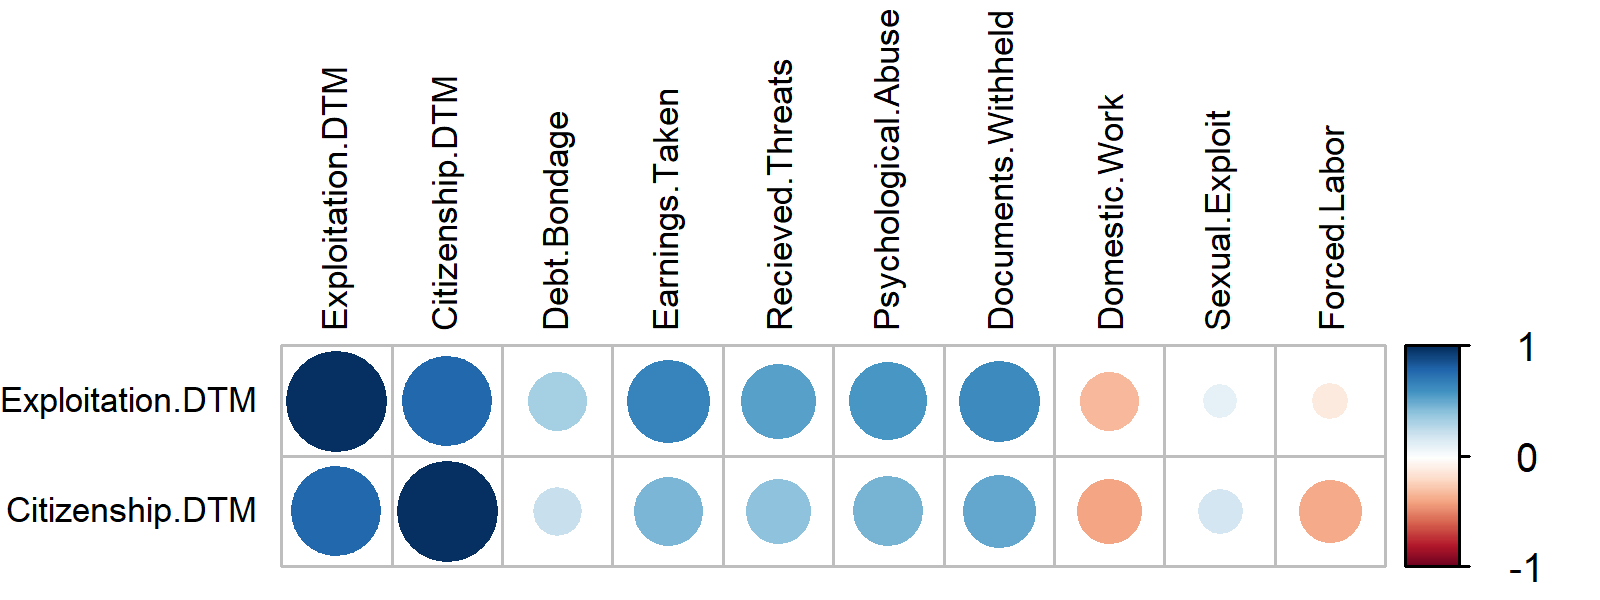
\includegraphics{Corrplot} \bigskip

Each of the variables included in the plot have at least a moderate correlation with DTM. As such, it would be beneficial to further quantify and model what types of relationships do exist within the data.

\section{Methods of Research}

The eventual goal of this research is to create a multinomial regression model. This is a probabilistic model which, for any given observation, it will give the probability of the observation being in a certain group. In our case, the groups will be the stage of development of a country in which a human trafficking victim is found. By creating a model of this type, we can analyze each coefficient for the predictors, and see what impact changing a predictor has on the predicted outcome. Thus, we can quantify just how much of a connection exists between stage of development, and certain predictors in our model.

The creation of this model will initially be done using a multinomial neural-network architecture to find which coefficients for predictors provide the least number of classifications on the data. If time permits, other model architectures will be tested to see if any of those perform better on our data set.


Perhaps the biggest hurdle to be overcome is the sheer lack of complete entries in the data set. As a result, the first steps of this research will involve analyzing what data is missing, and determining how to address that. By using visualizations and quantitative measurements, we can determine which observed values (predictors) are causing the most incomplete entire in our data. We can also determine which predictors are missing in conjunction with each other, and which ones are missing independently. By doing this, we can determine which variables we should remove first, and see if it gives us enough complete observations to create a helpful model.

To test the effectiveness of our model, we will randomly split our data into two groups: a group for training the model, and a group for testing the model. After training the model, we will simply input the observations for the test set, and see how accurately the model is able to classify the observations.

\section{Final Goals}

One of the simplest explanations for why law enforcement is unequipped to adequately address human trafficking is that they "[do] not have the time,
resources or expertise to address [the] problem," \parencite{LawResponse}. The goal of this research is to produce an understanding of the types of connections that exist between certain aspects of human trafficking and how developed an area is. This would allow policy makers to create policies which allow law enforcement to be more equipped to find victims of human trafficking as their country becomes more developed, or less developed, as is the case in countries with civil unrest and have been effected by natural disasters \parencite{bar2010}.


\printbibliography


\end{document}
